\documentclass[review]{acmart}

\usepackage{booktabs} % For formal tables

\settopmatter{printacmref=false} % Removes citation info after abstract
\renewcommand\footnotetextcopyrightpermission[1]{} % removes footnote with conference information in first column
\usepackage{fancyhdr}
 
\pagestyle{fancy}
\fancyhf{}
\lhead{Caplan \& Wazowski, Fall 2019}
\rfoot{\thepage}

%\pagestyle{plain} % removes running headers

% Use the "authoryear" citation style, and make sure citations are in [square brackets].
\citestyle{acmauthoryear}
\setcitestyle{square}

% A useful command for controlling the number of authors per row.
% The default value of "authorsperrow" is 2.
\settopmatter{authorsperrow=1}

\begin{document}

% Title. 
% If your title is long, consider \title[short title]{full title} - "short title" will be used for running heads.
\title{Semi-definite Programs for Optimal Quantum Algorithms}

% please leave the subtitle!
\subtitle{CSCI 701 Final Project, Middlebury College, Fall 2019}

% Authors.
\author{Michael Czekanski}
\affiliation{%
  \institution{Middlebury College}}

\author{R. Teal Witter}
 \affiliation{%
   \institution{Middlebury College}}

\maketitle

% a couple of paragraphs describing your project
\section*{Abstract}

In this paper we aim to find optimal bounds for the run time of quantum algorithms. Using existing research to frame this problem as a semi-definite programming (SDP) problem.

% the other sections
\section{Introduction}

Quantum computers have the potential to 
solve computationally difficult problems
faster and more efficiently than classical computers.
Since sufficiently large quantum computers do not yet exist,
we cannot compare the time it takes a quantum computer
to run an algorithm to the time it takes a classical computer
to run an equivalent algorithm.
Instead we rely on asymptotic run time that 
characterizes the time an algorithm will take in relation
to the size of the input.
In the study of quantum algorithms, it is often easier
and more elegant to describe an algorithm's query complexity.
Imagine a model where an algorithm is given access
to an input as a string of bits.
The query complexity of an algorithm is then the number
of bits the algorithm needs to reveal to determine a solution.
Query complexity is a lower bound for run time
(each query takes one time step);
however, run time can asymptotically outpace query complexity.

Consider the Boolean function OR.
An algorithm for the OR function returns 0 if
there are only 0's in the input string
and 1 if there are any 1's in the input string.
Classically, an algorithm must check that
every single bit of the input is a 0.
Then if there are $n$ bits in the input string
the classical algorithm's query complexity is $n$.
However, the quantum algorithm Grover's search
can solve the function OR in $\sqrt{n}$ queries \cite{grover1996fast}.

In the study of quantum algorithms,
we call the query complexity of the most efficient quantum
algorithm optimal.
Then when comparing quantum and classical algorithms,
we can say that the quantum algorithm is more
efficient than the classical algorithm in the sense
that the optimal quantum query complexity
is lower than the optimal classical query complexity.

Lee et al. show that optimal quantum query complexity
corresponds to the solution of a semidefinite program (SDP)
\cite{lee2011quantum}.
Reichardt reformulates the SDP into a more simple description 
\cite{reichardt2009span}.
We take Reichardt's formulation and convert it
to a standard definition found in Boyd \cite{boyd2004convex}.
We then implement an SDP solver to find the
quantum query complexity of arbitrary Boolean functions.
(While the SDP can solve any function,
we limit our scope to Boolean functions with
binary inputs and outputs).

CVXOPT and SDPA are both popular, existing convex optimization
libraries in Python \cite{cvxopt, SDPA}.
However, neither libraries easily support the standard form
of the SDP problem we are solving.
We instead turn to an alternating direction method (ADM).
Wen et al.'s algorithm efficiently exploits the 
sparsity of our SDP \cite{adm}.

Our goal is to create a tool that takes as input a 
natural number $n$ and a Boolean function 
$f: \{0,1\}^n \rightarrow \{0,1\}$. 
By solving Reichardt's SDP problem with
Wen et al.'s ADM algorithm,
we return the optimal quantum query complexity of
$f$. We hope that quantum algorithm researchers use
our tool to discover and verify optimal quantum
algorithms.
\section{Methodology}

Let us define the objective function $M$ as 


Nullam mollis in lectus vitae tempus. Nam pellentesque tincidunt leo id dapibus. Etiam in euismod diam. \cite{ceres-solver, Asaro:1976:POT} Phasellus feugiat ante et dui rhoncus, at dictum elit vehicula. Nunc ut finibus neque. Sed vehicula tristique - as shown in Table \ref{soccer} - odio at interdum. Morbi ex lectus, porttitor vel ipsum id, scelerisque facilisis metus. Cras orci sapien, luctus in eros in, suscipit rhoncus neque. Duis pharetra elit vitae sagittis maximus. Curabitur fermentum justo massa, sed placerat odio aliquam quis. Nam facilisis hendrerit ante eget maximus. Nulla et porttitor nibh, et malesuada turpis. Suspendisse potenti. Nunc ultricies suscipit quam, eget ultrices nisi viverra vitae.

\begin{table}[ht]
\begin{center}
    \caption{Soccer, or football?}
\label{soccer}
\begin{tabular}{l*{6}{c}r}
Team              & P & W & D & L & F  & A & Pts \\
\hline
Manchester United & 6 & 4 & 0 & 2 & 10 & 5 & 12  \\
Celtic            & 6 & 3 & 0 & 3 &  8 & 9 &  9  \\
Benfica           & 6 & 2 & 1 & 3 &  7 & 8 &  7  \\
FC Copenhagen     & 6 & 2 & 1 & 3 &  5 & 8 &  7  \\
\end{tabular}
\end{center}
\end{table}

Aliquam sed vehicula neque. Praesent placerat, nisi sit amet condimentum porta, justo tellus dictum eros, quis vestibulum erat massa id sapien. Vestibulum euismod purus dolor, ornare consectetur quam egestas volutpat. Curabitur sollicitudin convallis purus ultrices facilisis. Pellentesque sollicitudin maximus orci quis rutrum. Phasellus a mauris maximus sem mollis sagittis. Vivamus sagittis faucibus tincidunt. Vivamus vel suscipit leo.

\begin{figure}[h]
  \centering
  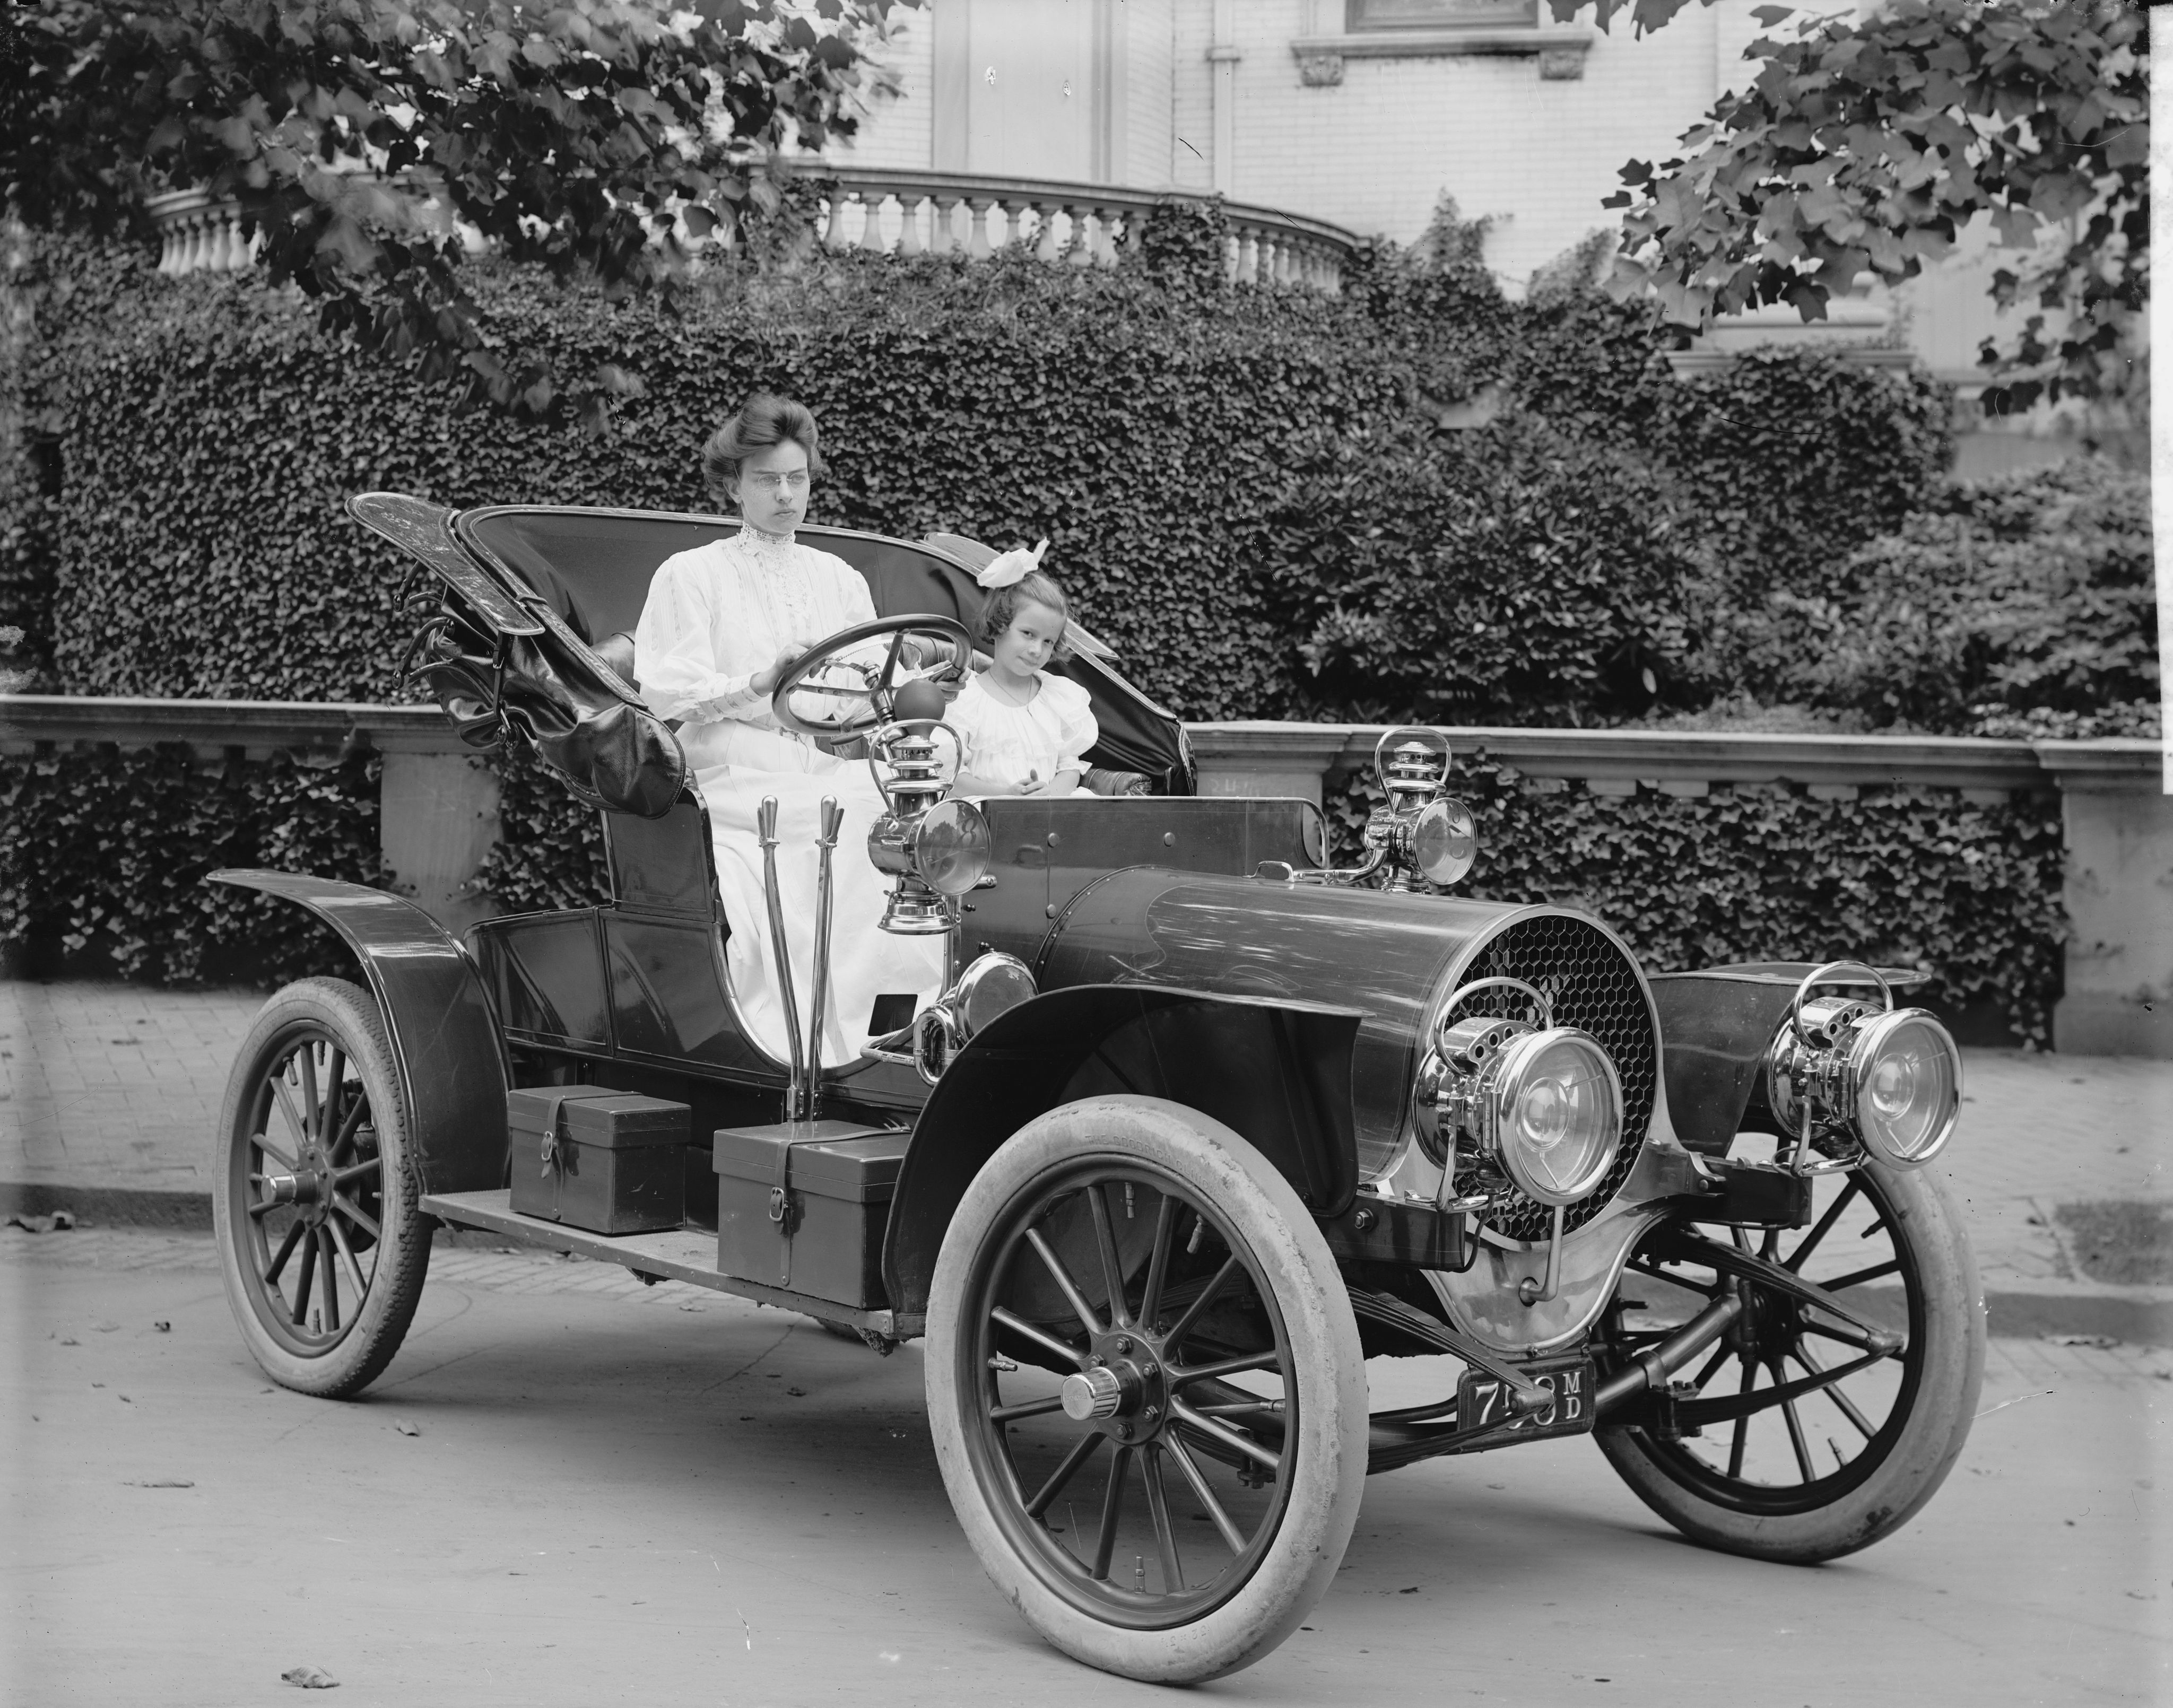
\includegraphics[width=\linewidth]{fig/franklin}
  \caption{1907 Franklin Model D roadster. Photograph by Harris \& Ewing, Inc. [Public domain], via Wikimedia Commons. (\url{https://goo.gl/VLCRBB}).}
\end{figure}
\subsubsection{Participants}

Cum sociis natoque penatibus et magnis dis parturient montes, nascetur ridiculus mus. Vivamus maximus a lectus sed dictum. Curabitur pulvinar lectus nec magna molestie consequat. Donec ligula urna, scelerisque et felis sed, euismod feugiat sem. (See equation \ref{eqn:01}.) Donec urna libero, auctor sit amet sem id, malesuada tempor risus. Morbi malesuada lobortis consequat. Aliquam lacinia quam ac tristique sodales. Class aptent taciti sociosqu ad 
\begin{equation}
\label{eqn:01}
P(t)=\frac{b^{\frac{t+1}{T+1}}-b^{\frac{t}{T+1}}}{b-1},
\end{equation}
where $t=0,{\ldots}\,,T$, and $b$ is a number greater than $1$, litora torquent per conubia nostra, per inceptos himenaeos.

\begin{multline}
\label{the-rendering-equation}
L_o(x, \omega_o, \lambda, t) = L_e(x, \omega_o, \lambda, t)  + \\
\int_{\Omega} f_r(x, \omega_i, \omega_o, \lambda, t) L_i(x, \omega_i, \lambda, t)(\omega_i \cdot n) \text{d} \omega_i
\end{multline}

Lorem ipsum dolor sit amet, consectetur adipiscing elit. Fusce auctor accumsan nulla, vitae pharetra ipsum sagittis sit amet. Donec ac metus consectetur, venenatis magna sit amet, viverra sapien. Class aptent taciti sociosqu ad litora torquent per conubia nostra, per inceptos himenaeos. Phasellus eleifend sem sit amet arcu congue tempus. Proin at iaculis orci. (See equation \ref{the-rendering-equation}.) Pellentesque habitant morbi tristique senectus et netus et malesuada fames ac turpis egestas. Orci varius natoque penatibus et magnis dis parturient montes, nascetur ridiculus mus. Etiam feugiat dui sit amet ante pellentesque, sed malesuada libero ornare. Curabitur tempor ligula leo, in feugiat urna ornare luctus. Fusce quis metus sit amet neque sagittis elementum. Quisque facilisis quam quis tortor volutpat, et sodales urna efficitur.
\section{Results}

We will make progress :)
\section{Changes to Scope}

The most obvious next step is to
speed up our SDP solver.
The slowest part of our implementation is the
process of decomposing a very large matrix at
each iteration.
While we will always need to implement
such a computationally expensive step,
we may save space and time by optimizing other 
components of our implementation.
We could increase the efficiency that
we store our matrices or otherwise 
decrease the computational work done at each step.
However, even in the best case where
we double or triple the speed of our implementation,
we are hitting the exponential size of the SDP.
A scalar improvement will not make a meaningful
difference in our ability to solve different sizes
of SDP.
Right now, we can solve SDPs on all bit strings
of length 4 or maybe 5 in reasonable time
but we will not be able to reasonably solve
SDPs with all 6 or 7 bit strings no matter the extent
to which we optimize our implementation.

Computationally we cannot make much progress.
But if we can limit the inputs to our SDP,
only considering the worst-case bit strings
of the Boolean function,
we can decrease the size of our SDP problem
and therefore the time it takes to solve.
As demonstrated in \cref{sec:speed}, 
the strategy of considering only the worst-case
inputs substantially improves the speed of solving the SDP.
One way we can limit the Boolean inputs is from
insights about the Boolean function.
We have demonstrated this approach in perhaps the most
trivial case with OR.
We can extend this strategy by considering additional
Boolean functions.
The other, more general way we can limit the number
of Boolean inputs is by optimizing our SDP solver.
Perhaps within a few iterations, we can tell
that certain inputs take relatively few queries to find
the output.
By optimizing as we go, we can apply our strategy to
an Boolean function while simultaneously cutting down
the time run time of solving it.

Another direction for our work is to implement
a distinct but related problem.
Our SDP solver solves the primal:
finding the optimal quantum query complexity
of arbitrary Boolean functions)
There also exists a dual SDP whose solution 
corresponds to the optimal quantum algorithm itself.
We can implement the dual of our current problem
and, in addition to finding the query complexity,
also find the algorithm itself.



\begin{acks}
The authors would like to thank Professors Shelby Kimmel
and Philip Caplan for their invaluable help and support. 
\end{acks}

% select the reference format (leave this)
\bibliographystyle{ACM-Reference-Format}

% specify the bibliography (.bib) file
% place your references in this bib file
\bibliography{main}

\end{document}